
\begin{frame}
  \frametitle{Nested Components}
  The NuclideModel in a Component can be interchangeably represented by any of 
  the four nuclide transport models. 
    \begin{itemize}
      \item Degradation Rate Based Failure Model
      \item Mixed Cell with Degradation, Sorption, Solubility Limitation
      \item Lumped Parameter Model
      \item 1D van Genuchten Advection Dispersion Solution
    \end{itemize}
\end{frame}

\begin{frame}
\frametitle{Clay GDSM Model}
\begin{figure}[htbp!]
  \begin{center}
    \includegraphics[width=0.9\textwidth]{./images/clay_gdsm.eps}
  \end{center}
  \caption{The Clay Generic Disposal System Model (GDSM) was used for 
  preliminary sensitivity analysis, abstraction iteration, and validation.
  This figure was reproduced from Figure 3.3-2 in \cite{clayton_generic_2011}.}
  \label{fig:clay_gdsm}
\end{figure}

\end{frame}

\begin{frame}
  \frametitle{Advection Dispersion Equation}
  \footnotesize{
    In a saturated, reducing environment, contaminants are transported by 
    \textbf{dispersion} and \textbf{advection} 
    \cite{schwartz_fundamentals_2004, 
    wang_introduction_1982, van_genuchten_analytical_1982}: 
    \begin{align}
      J &= J_{dis} + J_{adv}\nonumber\\
      &= -\theta(D_{mdis} + \tau D_m)\nabla C + \theta vC\nonumber\\ 
      &= -\theta D\nabla C + \theta vC \nonumber\\ 
      \label{unidirflow}
      \intertext{where}
      J_{dis} &= \mbox{ Total Dispersive Mass Flux }[kg/m^2/s]\nonumber\\
      J_{adv} &= \mbox{ Advective Mass Flux }[kg/m^2/s]\nonumber\\
      \tau &= \mbox{ Toruosity }[-] \nonumber\\
      \theta &= \mbox{ Porosity }[-] \nonumber\\
      D_m &= \mbox{ Molecular diffusion coefficient }[m^2/s]\nonumber\\
      D_{mdis} &= \mbox{ Coefficient of mechanical dispersivity}[m^2/s]\nonumber\\
      D &= \mbox{ Effective Dispersion Coefficient }[m^2/s]\nonumber\\
      C &= \mbox{ Concentration }[kg/m^3]\nonumber\\
      v &= \mbox{ Fluid Velocity in the medium }[m/s].\nonumber
    \end{align}
    }

\end{frame}

%\begin{frame}
%  \frametitle{Component Interfaces}
%  \footnotesize{
%Solutions to this equation can be categorized by their boundary conditions and 
%those boundary conditions serve as the interfaces between components in the 
%Cyder library of nuclide transport models.
%
%  \begin{figure}[htp!]
%    \begin{center}
%      \def\svgwidth{\textwidth}
%      \input{images/flow.eps_tex}
%    \end{center}
%    \caption{The boundaries between components are robust interfaces defined by 
%    Source Term, Dirichlet, Neumann, and Cauchy boundary conditions.}
%    \label{fig:flow}
%  \end{figure}
%  }
%\end{frame}

\begin{frame}
\frametitle{Timestepping Algorithm}

\begin{figure}[htbp!]
  \begin{center}
    \def\svgwidth{.5\textwidth}
    \input{images/vols.eps_tex}
  \end{center}
  \caption{Two components share an interface at $r_k$ and contain mass and 
  concentration profiles at the beginning of timestep $t_n$.}
  \label{fig:vols}
\end{figure}

\end{frame}
\begin{frame}
\frametitle{Timestepping Algorithm}

\begin{figure}[htbp!]
  \begin{center}
    \def\svgwidth{.5\textwidth}
    \input{images/vols_trans.eps_tex}
  \end{center}
  \caption{The mass balance model in component k calculates the appropriate 
  mass transfer based on boundary information from component j.}
  \label{fig:vols_trans}
\end{figure}

\end{frame}
\begin{frame}
\frametitle{Timestepping Algorithm}

\begin{figure}[htbp!]
  \begin{center}
    \def\svgwidth{.5\textwidth}
    \input{images/vols_update.eps_tex}
  \end{center}
  \caption{Based on the mass transfer, both components update their mass and 
  concentration profiles based on their mass balance model.}
  \label{fig:vols_update}
\end{figure}

\end{frame}


%\begin{frame}
%  \frametitle{Radionuclide Transport: Degradation Rate Based Release}
%  \footnotesize{
%In this model, the contaminants in the degraded fraction of the control volume 
%are available to adjacent components. The available contaminants
%$m_{ij}(t)$, at the boundary between cell $i$ to cell $j$ at time $t$ are thus

%\begin{align}
%\dot{m}_{ij}(t) &= f_im_i(t)
%\label{deg_rate_source_cont}
%\intertext{where}
%\dot{m}_{ij} &= \mbox{ the rate of mass transfer from i to j }[kg/s]\nonumber\\
%f_i &= \mbox{ degradation rate function in cell i }[1/s] \nonumber\\
%m_i &= \mbox{ mass in cell i }[kg] \nonumber\\
%t &= \mbox{ time  }[s].\nonumber
%\end{align}
%}
%\end{frame}


\begin{frame}
  \frametitle{Radionuclide Transport: Degradation Rate Based Release}
  \begin{figure}[h!]
  \begin{center}
    \def\svgwidth{.7\textwidth}
    \begin{figure}[h!]
  \begin{center}
    \def\svgwidth{.7\textwidth}
    \begin{figure}[h!]
  \begin{center}
    \def\svgwidth{.7\textwidth}
    \input{./chapters/methodology/nuclide_models/mass_balance/deg_rate/deg_volumes.eps_tex}
  \end{center}
  \caption[Constituents of a Degradation Rate Control Volume]{The control volume contains an 
  intact volume $V_i$ and a degraded volume, $V_d$. Contaminants in $V_d$ are 
  available for transport, while contaminants in $V_i$ are contained.}
  \label{fig:deg_volumes}
\end{figure}


  \end{center}
  \caption[Constituents of a Degradation Rate Control Volume]{The control volume contains an 
  intact volume $V_i$ and a degraded volume, $V_d$. Contaminants in $V_d$ are 
  available for transport, while contaminants in $V_i$ are contained.}
  \label{fig:deg_volumes}
\end{figure}


  \end{center}
  \caption[Constituents of a Degradation Rate Control Volume]{The control volume contains an 
  intact volume $V_i$ and a degraded volume, $V_d$. Contaminants in $V_d$ are 
  available for transport, while contaminants in $V_i$ are contained.}
  \label{fig:deg_volumes}
\end{figure}


\end{frame}

\begin{frame}
  \frametitle{Radionuclide Transport : Mixed Cell with Sorption and Solubility}
  \begin{figure}[h!]
  \begin{center}
    \def\svgwidth{\textwidth}
    \begin{figure}[h!]
  \begin{center}
    \def\svgwidth{\textwidth}
    \begin{figure}[h!]
  \begin{center}
    \def\svgwidth{\textwidth}
    \input{./images/deg_sorb_volumes.eps_tex}
  \end{center}
  \caption[Constituents of a Mixed Cell Control Volume]{The degraded volume is 
  modeled as a solid degraded volume, $V_{ds}$, and a fluid degraded volume, 
  $V_{df}$. The intact volume is modeled as an intact solid volume, $V_{is}$, and 
  an intact fluid volume $V_{if}$.  Only contaminants in $V_{df}$ are available 
  for transport.}
  \label{fig:deg_sorb_volumes}
\end{figure}


  \end{center}
  \caption[Constituents of a Mixed Cell Control Volume]{The degraded volume is 
  modeled as a solid degraded volume, $V_{ds}$, and a fluid degraded volume, 
  $V_{df}$. The intact volume is modeled as an intact solid volume, $V_{is}$, and 
  an intact fluid volume $V_{if}$.  Only contaminants in $V_{df}$ are available 
  for transport.}
  \label{fig:deg_sorb_volumes}
\end{figure}


  \end{center}
  \caption[Constituents of a Mixed Cell Control Volume]{The degraded volume is 
  modeled as a solid degraded volume, $V_{ds}$, and a fluid degraded volume, 
  $V_{df}$. The intact volume is modeled as an intact solid volume, $V_{is}$, and 
  an intact fluid volume $V_{if}$.  Only contaminants in $V_{df}$ are available 
  for transport.}
  \label{fig:deg_sorb_volumes}
\end{figure}


\end{frame}

\begin{frame}
  \frametitle{Radionuclide Transport : Mixed Cell Sorption}
The mass of contaminant sorbed into the degraded and precipitated solids can be
found using a linear isotherm model \cite{schwartz_fundamentals_2004},
characterized by the relationship 
\begin{align}
s_{i} &= K_{di} C_{i}
\label{linear_iso}
\intertext{where}
s_i &= \mbox{ the solid concentration of isotope i }[kg/kg]\nonumber\\
K_{di} &= \mbox{ the distribution coefficient of isotope i}[m^3/kg]\nonumber\\
C_i &= \mbox{ the liquid concentration of isotope i }[kg/m^3].\nonumber
\end{align}
\end{frame}

\begin{frame}
  \frametitle{Radionuclide Transport : Mixed Cell Solubility Limitation}
  \footnotesize{
In addition to engineered barriers, contaminant transport is constrained by 
  the solubility limit \cite{hedin_integrated_2002}, 
    \begin{align}
      m_{s,i} &\leq V_w C_{sol,i},
    \intertext{where}
      m_{s,i} &= \mbox{ solubility limited mass of isotope i in volume }V_w [kg]\nonumber\\ 
      V_w &= \mbox{ volume of the solution }[m^3]\nonumber\\
      C_{sol,i} &= \mbox{ solubility limit, the maximum concentration of i }[kg/m^3].\nonumber
    \end{align}

\end{frame}

\begin{frame}
  \frametitle{Radionuclide Transport: Lumped Parameter Transport Model}
\footnotesize{
\begin{figure}[htbp!]
  \begin{center}
    \def\svgwidth{\textwidth}
    \input{images/lumpedseries.eps_tex}
  \end{center}
  \caption{ The method by which each lumped parameter component is modeled is
according to a relationship between the incoming concentration, $C_{in}(t)$,
and the outgoing concentration, $C_{out}(t)$.}
  \label{fig:lumpedseries}
\end{figure}

\begin{align}
  C_{out}(t) &= \int_0^\infty C_{in}(t-t')g(t')e^{-\lambda t'}dt'
  \label{lumped2}
  \intertext{where}
  t'  &= \mbox{ time of entry }[s]\nonumber\\
  t-t'  &= \mbox{ transit time }[s]\nonumber\\
  g(t-t')  &= \mbox{ response function, a.k.a. transit time distribution}[-]\nonumber\\
  \lambda &= \mbox{ radioactive decay constant}[s^{-1}].\nonumber
\end{align}
}
\end{frame}

\begin{frame}
  \frametitle{Radionuclide Transport: Lumped Parameter Transport Model}
\footnotesize{
Selection of the response function is usually based on experimental tracer
results in the medium at hand. However, some functions used commonly in
chemical engineering applications \cite{maloszewski_lumped_1996} include the
Piston Flow Model (PFM), 
\begin{align}
  g_{PFM}(t') &= \delta{(t'-t_t))}
  \intertext{ the Exponential Model (EM) }
  g_{EM}(t') &= \frac{1}{t_t}e^{-\frac{t'}{t_t}}
  \intertext{ and the Dispersion Model (DM), }
  g_{DM}(t') &= \left( \frac{\text{Pe }t_t}{4\pi t'} \right)^{\frac{1}{2}}
  \frac{1}{t'}e^{- \frac{\text{Pe }t_t\left( 1- \frac{t'}{t_t}  \right)^2} 
  {4t'}}, \intertext{where}
  \text{Pe}  &= \mbox{ Peclet number for mass diffusion }[-]\nonumber\\
  t_t  &= \mbox{ mean tracer age }[s]\nonumber\\
    &= t_w \mbox{ if there are no stagnant areas }\nonumber\\
  t_w  &= \mbox{ mean residence time of water }[s]\nonumber\\
       &= \frac{V_m}{Q}\nonumber\\
       &= \frac{z}{v_z}\nonumber\\
       &= \frac{z\theta_e}{q}\nonumber
  \intertext{in which}
  V_m  &= \mbox{ mobile water volume }[m^3]\nonumber\\
  Q    &= \mbox{ volumetric flow rate }[m^3/s]\nonumber\\
  z    &= \mbox{ average travel distance in flow direction }[m]\nonumber\\
  v_z  &= \mbox{ mean water velocity}[m/s]\nonumber\\
  q    &= \mbox{ Darcy Flux }[m/s]\nonumber\\
  \theta_e &= \mbox{ effective (connected) porosity }[\%].\nonumber
\end{align}
}
\end{frame}

\begin{frame}
  \frametitle{Radionuclide Transport: Lumped Parameter Transport Model}
\footnotesize{
The solutions to these for constant concentration at the 
source boundary are given in \cite{maloszewski_lumped_1996}, 
\begin{align}
  C(t) &=\begin{cases}
    PFM & C_0e^{-\lambda t_t}\\
    EM  & \frac{C_0}{1+\lambda t_t}\\
    DM & C_0e^{\frac{\texttt{Pe}}{2}\left(1-\sqrt{1+\frac{4\lambda 
    t_t}{\texttt{Pe}}}\right)}.
  \end{cases}
  \label{lumpedsolns}
\end{align}
}
\end{frame}


\begin{frame}
  \frametitle{Radionuclide Transport: 1D Finite, Cauchy B.C.}
  \footnotesize{
\begin{figure}[htbp!]
  \begin{center}
    \def\svgwidth{.5\textwidth}
    \input{images/1dfin.eps_tex}
  \end{center}
  \caption{A one dimensional, finite, unidirectional flow,
  solution with Cauchy and Neumann boundary conditions}
  \label{fig:1dinf}
\end{figure}
}
\end{frame}

\begin{frame}
  \frametitle{Radionuclide Transport: 1D Finite, Cauchy B.C.}
For the boundary conditions, 
\begin{align}
  -D \frac{\partial C}{\partial z}\big|_{z=0} + v_zc &= \begin{cases}
    v_zC_0  &  \left( 0<t<t_0 \right)\\
    0  &  \left( t>t_0 \right)\\
  \end{cases}
\intertext{and}
  \frac{\partial C}{\partial z}\big|_{z=L} &= 0
  \intertext{and the initial condition,}
  C(z,0) &= C_i,
  \label{1dinfBC}
  \intertext{the solution is given as }
  C(z,t) &= \begin{cases} 
  C_i + \left(C_0 - C_i\right)A\left(z,t\right) & 0<t\le t_0\\
  C_i + \left(C_0 - C_i\right)A\left(z,t\right) - C_0A(z,t-t_0) & t\ge t_0.
  \end{cases}
\end{align}
\end{frame}

\begin{frame}
  \frametitle{Radionuclide Transport: 1D Finite, Cauchy B.C.}
\footnotesize{For the vertical flow coordinate system, $A$ is defined as
\begin{align}
A(z,t) =& \left(\frac{1}{2}\right)\erfc{\left[\frac{Rz-vt}{2\sqrt{DRt}}\right]} \nonumber\\
&+ \left(\frac{v^2t}{\pi RD}\right)^{1/2}\exp{\left[-\frac{(Rz-vt)^2}{4DRt}\right]}\nonumber\\ 
&- \frac{1}{2} \left(1+\frac{vz}{D} + \frac{v^2t}{DR}\right) \exp{\left[\frac{vz}{D}\right]}\erfc{\left[\frac{Rz+vt}{2\sqrt{DRt}}\right]}\nonumber\\
&+ \left(\frac{4v^2t}{\pi RD}\right)^{1/2}\left[1+\frac{v}{4D}\left(2L-z+\frac{vt}{R}\right)\right]\exp{\left[\frac{vL}{D} - \frac{R}{4Dt}\left(2L-z+\frac{vt}{R}\right)^2\right]}\nonumber\\
&- \frac{v}{D}\left[2L - z + \frac{3vt}{2R} + \frac{v}{4D}\left(2L - z + \frac{vt}{R}\right)^2\right]\exp{\left[\frac{vL}{D}\right]}\erfc{\left[\frac{R(2L-z) + vt}{2\sqrt{DRt}}\right]}\nonumber
\intertext{where}
L =& \mbox{Extent of the solution domain }[m]\nonumber\\
R =& \mbox{Retardation factor }[-].\nonumber
\end{align}
}
\end{frame}
